%!TEX root=../../../main.tex

While annotations facilitate individual note taking for users and improve
engagement inside platforms deploying such mechanisms, it is also desirable
that metadata can be shared across ecosystems in order to allow for new
connections between information resources to be established. Thus, the usage of
standardised annotation dissemination formats is necessary.

The systems presented in the previous subsection make use of different forms of
RDF structures in order to represent annotations both internally and
externally.  RDF, or the Resource Description Framework \cite{ref:rdf} is a
model defined by the World Wide Web Consortium (W3C) to be used for online data
interchange. The main idea behind it is related to making statements about
resources in the form of subject-predicate-object expressions, such as:

\begin{verbatim}
  <Dave Beckett> <edits> <the RDF syntax grammar specification>
\end{verbatim}

Due to this structure, these statements are named \textit{triples} in the RDF
terminology.  A collection of RDF statements will constitute a directed
multi-graph, also named the \textit{context} of the concerned triples. A simple
example is shown in Fig. \ref{fig:rdf}

\begin{figure}[!ht]
  \centering
  \fbox{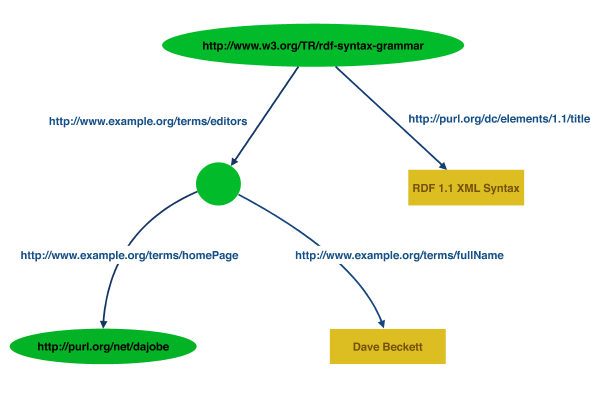
\includegraphics[scale=1]{static/img/rdf.png}}
  \caption[Example RDF graph]
          {Example RDF graph, source \cite{ref:rdfsyntax}. This graph
           can be summarised briefly as: The RDF syntax specification, identified by a
           URL, has a person identified by its full name and personal Web page
           as editor.}
  \label{fig:rdf}
\end{figure}

It can be observed that this model is very well-suited for the annotations use
case. Metadata can be seen as a statement about a resource in the form (but not
restricted to):

\begin{verbatim}
  <Resource identified by URL/ URI> <has metadata> <annotation body text>
\end{verbatim}

The RDF data model can be serialised in different formats, such as Turtle,
N-Triples, N-Quads (a superset of N-Triples), Notation 3 (N3), RDF/XML or
JSON-LD. Note that the RDF/XML format is commonly referred as simply RDF, due
to its widespread usage, leading to some confusion between the \textit{data
  model} and the \textit{serialisation format}. A typical RDF/XML document will
look as the one in Figure \ref{lst:rdf}, which encodes the graph in Fig.
\ref{fig:rdf}. In order to be encoded in XML, the RDF graph nodes and
predicates need to be represented in the specific XML structural terms: element
and attribute names, element contents and attribute values. Note that the
example XML uses three collections to define the elements, namely the RDF
standard set, the Dublin Core Metadata Element Set \cite{ref:dc} and a
placeholder set; in real use-cases, each Web application can define its own set
of elements, depending on the specific domain knowledge.

\begin{figure}[!ht]
  \lstinputlisting[language=XML,
                   frame=tb,
                   captionpos=b,
                   numbers=none,
                   showspaces=false,
                   showstringspaces=false,
                   showtabs=false,
                   stepnumber=2,
                   numbersep=4pt]
    {static/lst/rdf.xml}
    \caption[RDF/XML Example]
            {RDF/XML Example, source \cite{ref:rdfsyntax}}
    \label{lst:rdf}
\end{figure}

Similar to the RDF/XML, an augmented version of the JavaScript Object Notation
(JSON) format, JSON-LD, can also be used to serialise the data model; an
in-detail description, in the usage context of the project is included in
Section \ref{sec:json}.

Relational databases, while not suitable for the graph structure of the RDF
model, are the most used solution for storing such data. If a database stores
only the triples it is called a \textit{triplestore}, and if the context is
also included, a \textit{quad} store is employed. These stores can be queried
using the SPARQL \cite{ref:sparql} language.

While RDF provides a standard method for disseminating data, it is mainly
purposed for machine manipulation. Taking the RDF/XML format as an example, it
can be seen that editing such a document by hand is not optimal for end-users.
On the other hand, capturing input and filling a XML template, while accounting
for invalid data or out-of-scope information, can become expensive in terms of
computing resources.

A simple solution is to deploy standard forms for guiding the users in the data
collection process. The Pundit project discussed previously uses such a form
for allowing users to input RDF statements. While this solution is fast to
develop due to the prevalence of the practice in Web applications, it also
lacks in terms of extensibility and scalability; it can be seen that in order
to be able to express complex RDF graphs, a considerable effort must be
invested.

The XTiger \cite{ref:xtiger} XML language allows defining templates, in order
to guide an editing tool for building documents that follow a predefined model.
It does this by predefining a set of typed structures and constructors for
these (\textit{components}); for example, a minimal template for inputting
annotations could be defined as in Figure \ref{lst:xtiger}. The XTiger template
can be used to generate documents in a target language, for example XHTML or
RDF/XML.

\begin{figure}[!ht]
  \lstinputlisting[language=XML,
                   frame=tb,
                   captionpos=b,
                   numbers=none,
                   showspaces=false,
                   showstringspaces=false,
                   showtabs=false,
                   stepnumber=2,
                   numbersep=4pt]
    {static/lst/xtiger.xml}
  \caption[XTiger template fragment for annotation input]
            {XTiger template fragment for annotation input. A custom component,
             consisting of two input fields, is defined in the \texttt{xt:head}
             element and used to build the form inside the XHTML body.}
  \label{lst:xtiger}
\end{figure}

Special constructs for repeating components across the resulting document can
ease the creation of complex structures. RDF graphs can be constructed by using
the RDF/XML serialisation format as the target for a XTiger template and by
leveraging the special constructs that allow repeating components across the
produced document (e.g., \texttt{xt:repeat}). It is worth noting that XTiger
borrows certain elements from XML Schema, being possible to define the
semantics of XTiger as an extension of XML Document Type Definitions (DTD);
thus the constraints defined by a XTiger template can be expressed in schema
language and a XSLT transformation can be employed to perform the translation
to XML Schema \cite{ref:quint}.

To allow even further flexibility, the Adaptable XML Editing Library (AXEL)
\cite{ref:axel} can be used. This JavaScript library allows users to freely
combine XTiger components, while still producing conforming documents as the
end-result.

Another possibility is to use RDFa \cite{ref:rdfa}, a specification for
attributes to express structured data in any markup language. For example, RDF
attributes can be inserted into the XHTML documents used to present and capture
metadata, facilitating the annotation workflow from both the perspective of the
end-user and the backend system.
